% !TEX root = ../analisis.tex

%=========================================================
\section{Módulos del sistema}

    El sistema se encuentra organizado en dos  módulos con la finalidad de agrupar y administrar de mejor manera los requerimientos funcionales del sistema. Dividir el sistema en dos módulos permite visualizar e identificar rápidamente aquellos aspectos funcionales que pueden tratarse conjuntamente. \\

%    La figura \ref{fig:ModulosPAEAR} muestra los módulos propuestos de manera inicial para el \saear. Cada uno de estos módulos agrupan los casos de uso que poseen funcionalidad similar o que trabajan en conjunto para alcanzar un aspecto funcional del sistema. Cada uno de los módulos que se muestran en la figura se describen a continuación:

%    \begin{figure}[h!]
%	\begin{center}
%	      \fbox{\includegraphics[width=\textwidth]{images/modulos.jpg}}
%	\caption{Módulos del \saear.}
%	\label{fig:ModulosPAEAR}
%	\end{center}
%    \end{figure}

    \begin{itemize}
	\item {\bf Consulta de profesores:} Agrupa los casos de uso que tienen que ver con la consulta de profesores de la ESCOM. 

	%\item {\bf Proceso de inscripción} Agrupa los casos de uso que permiten a los aspirante aceptados, así como a los alumnos de semestres arriba poder inscribirse a un nuevo ciclo escolar.
	
	\item {\bf Horarios:} Agrupa los casos de uso que tienen que ver con la creación y confirguación de horarios.
%	
%	\item {\bf Proceso de estructuración académica:} Agrupa los casos de uso que tienen que ver con el proceso de estructuración académica de la Escuela Libre de Derecho. 
    \end{itemize}

%=========================================================
\section{Actores del sistema}\label{sec:Comportamiento:ActoresSistema}

Los actores son los perfiles asociados a las diversas personas que intervienen en la aplicación. Se han identificado los actores de acuerdo a las actividades y responsabilidades que obtienen al ser usuarios de la aplicación, los cuales se muestran y se describen a continuación.

%    \begin{figure}[h!]
%      \begin{center}
%	  \includegraphics[width=0.6\textwidth]{images/actores/Actores.png}
%      \caption{Perfiles identificados.}
%      \label{fig:perfilesPAEAR}
%      \end{center}
%    \end{figure}

%ADMINISTRADOR
    \cdtLabel{Actor:Administrador}{}
    \begin{actor}{Administrador}{}{Persona que podrá gestionar la información de la ESCOMapp, es decir tendrá permisos para modificar la información de los profesores, así como los catálogos de las ubicaciones de edificios, salones, cubículos, etc. para que los alumnos puedan registrar la ubicación de sus salones, así como agregar una ubicación a los profesores.}

	\item[Área:] Persona que puede se interna o externa a la ESCOM.

	\item[Responsabilidades:] \hspace{1pt}
	
		\begin{itemize}
		    \item Poblar la BD, con información pública de los profesores.
		    \item Validar en su mayor parte posible la veracidad de la información que se registre.
		 \end{itemize}
		 
	\item[Perfil:] \hspace{1pt}
		\begin{itemize}
		    \item Persona con conocimientos en BD.
		    \item Persona con conocimientos en el manejo de la App.
	    \end{itemize}
	    
	\item[Cantidad:] Uno.
\end{actor}


%PROFESOR
\cdtLabel{Actor:Profesor}{}
\begin{actor}{Profesor}{}{Persona asignada a una Unidad de Aprendizaje en el Instituto para impartir cátedra a quienes los alumnos podrán visualizar la información para poder realizar consultas u otras actividades extra-curriculares.}

	\item[Área:] Profesor-Docente-Administrativo.
	
	\item[Responsabilidades:] \hspace{1pt}
	
	    \begin{itemize}
	    	\item Creación y manejo de cuenta personal.
	    	\item Mantener su información pública y no pública actualizada.
	    	\item Dar privilegios a la información no publica.
	    \end{itemize}
	    
	\item[Perfil:] Maestro en su área de conocimiento.
	
	\item[Cantidad:] No se define.
	
\end{actor}


%ALUMNO
\cdtLabel{Actor:Alumno}{}
\begin{actor}{Alumno}{-----}{Persona que posee un número de boleta que se identifica como Alumno de la Institución quien podrá registrar su horario en la aplicación y gestionar la ubicación donde se imparten las Unidades de Aprendizaje en las que esta inscrito.}
	
	\item[Área:] Secretaría de Administración - Control Escolar.
	
	\item[Responsabilidades:] \hspace{1pt}
	
	\begin{itemize}
		\item Creación y manejo de cuenta personal.
		\item Manejo de la información sobre los profesores y Horarios.
	\end{itemize}
	
	\item[Perfil:] Alumno de la ESCOM.

	\item[Cantidad:] No se define.
	
\end{actor}



%INVITADO
\cdtLabel{Actor:Invitado}{}
\begin{actor}{Invitado}{-----}{Persona externa al Instituto que podrá consultar la información publica de los Docentes.}
	
	\item[Área:] No se define.
	
	\item[Responsabilidades:] \hspace{1pt}
	
	\begin{itemize}
		\item Creación y manejo de cuenta personal.
		\item Manejo de la información sobre los profesores y Horarios.
	\end{itemize}
	
	\item[Perfil:] No se define.
	
\end{actor}




%====================================================================================
\section{Casos de Uso del módulo de Consulta de Profesores}

La figura \ref{fig:casosUso:generacionCalendario} muestra los casos de uso que integran la funcionalidad del módulo de \textbf{Consulta de Profesores}, que se refieren a la visualización de la información de los profesores de la ESCOM.

\begin{figure}[h!]
	\begin{center}
		\fbox{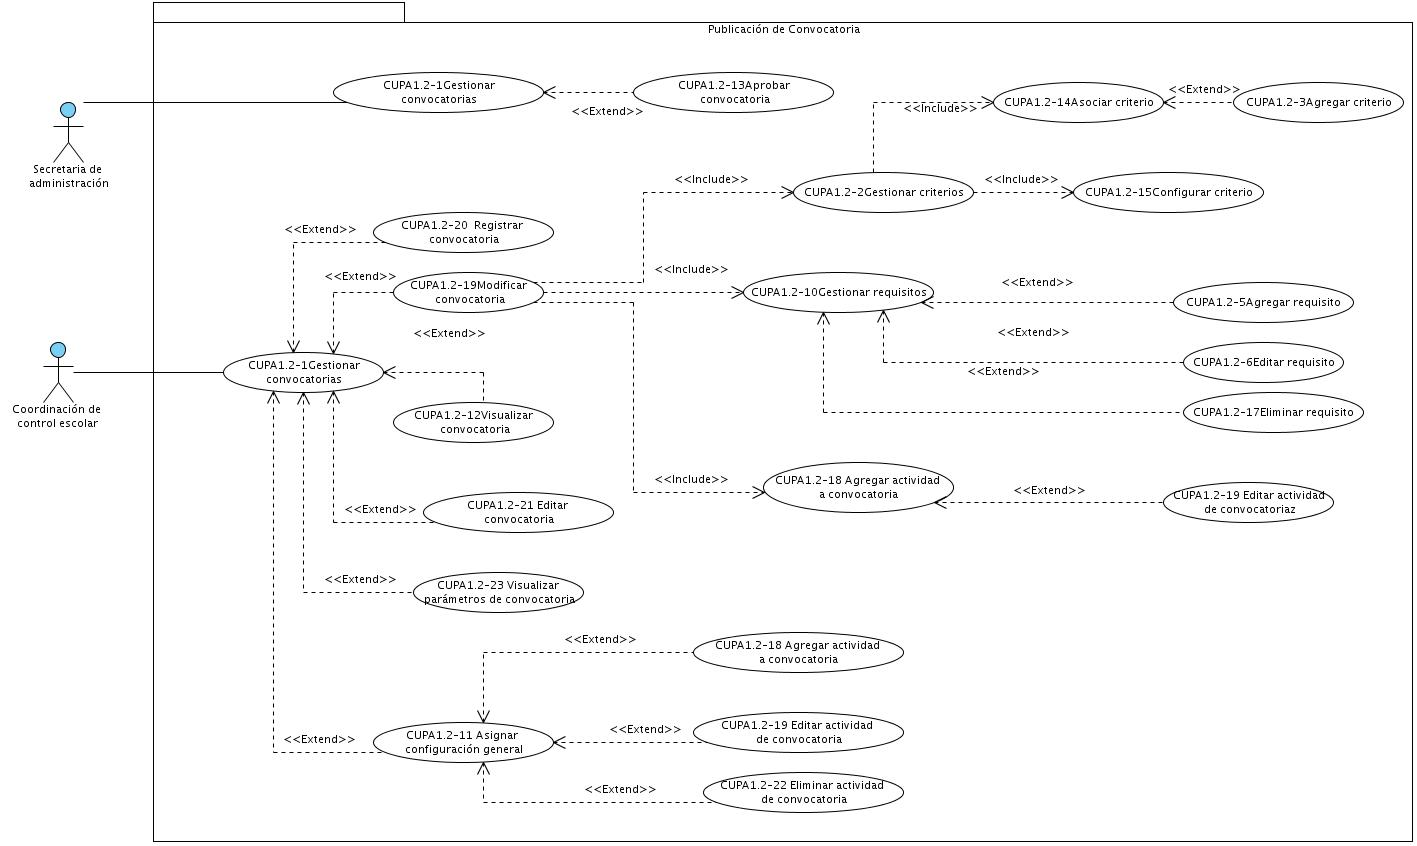
\includegraphics[width=.9\textwidth]{ModeloComportamiento/modulo-consultaDeProfesores/images/DCU_consulta_de_profesores}}
		\caption{Diagrama de casos de uso para el módulo de Consulta de profesores. \label{fig:casosUso:generacionCalendario}}
	\end{center}
\end{figure}

%====================================================================================
\section{Casos de Uso del módulo de Horarios}

La figura \ref{fig:casosUso:generacionConvocatoria} muestra los casos de uso que integran la funcionalidad del módulo de \textbf{Horarios}, que se refieren al registro, modificación y visualización los horarios que el \cdtRef{Actor:Alumno}{Alumno} o \cdtRef{Actor:Invitado}{Invitado}  registre en su cuenta personal.

\begin{figure}[h!]
	\begin{center}
		\fbox{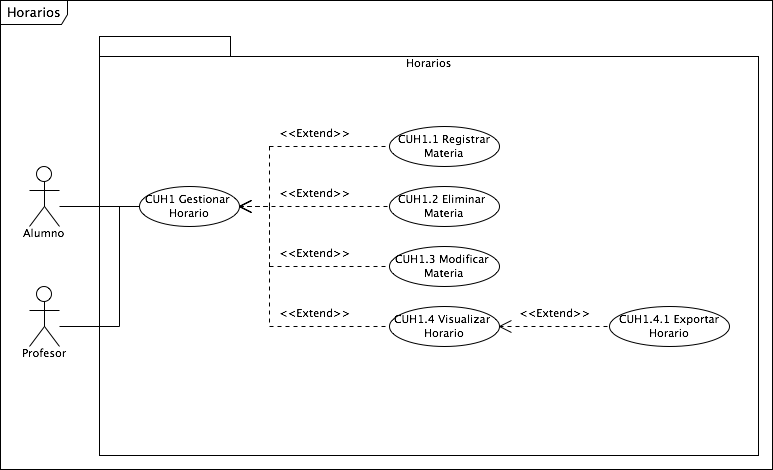
\includegraphics[width=.9\textwidth]{ModeloComportamiento/modulo-horarios/images/DCU_horarios}}
		\caption{Diagrama de casos de uso para el módulo de Horarios. \label{fig:casosUso:generacionConvocatoria}}
	\end{center}
\end{figure}
